\subsection{Stavový diagram}

%% State Machine Diagram - popis, časté použití, příklad

%%%%%%%%%%%%%%%%%%%%%%%%%%%%%%%%%%%%%%%%%%%%%%%%%%%%%%%%%%%%%%%%%%%%%%%%
%% Slide

\begin{frame}{Modelování stavů}

Stavový diagram (State Machine Diagram)

\begin{itemize}
	\item Modeluje komplexní životní cyklus některých elementů
	\item Popisuje stavy a přechody mezi stavy
	\item Konečné stavové automaty
	\item Stav (State)
	\item Přechod (Transition)
	\begin{itemize}
		\item Spouštěč (Trigger)
		%~ \begin{itemize}
			%~ \item Nějaká událost
			%~ \item Vyvolané někým
			%~ \item Něčím (automaticky) - např. časová událost, událost
			%~ změny, dokončení...
		%~ \end{itemize}
		\item Podmínka (Guard condition)
		\item Akce (Action)
	\end{itemize}
\end{itemize}

Co na diagramu najdeme

\begin{itemize}
	\item Počáteční stav
	\item Koncový stav
	\item Přechody (šipky)
	\item Spouštěče a akce jako popisky
	\item Další podmínky
\end{itemize}

\end{frame}

%%%%%%%%%%%%%%%%%%%%%%%%%%%%%%%%%%%%%%%%%%%%%%%%%%%%%%%%%%%%%%%%%%%%%%%%
%% Slide

\begin{frame}{Příklad}
Jednoduchý bug tracking systém - instance třídy Bug
\begin{figure}
	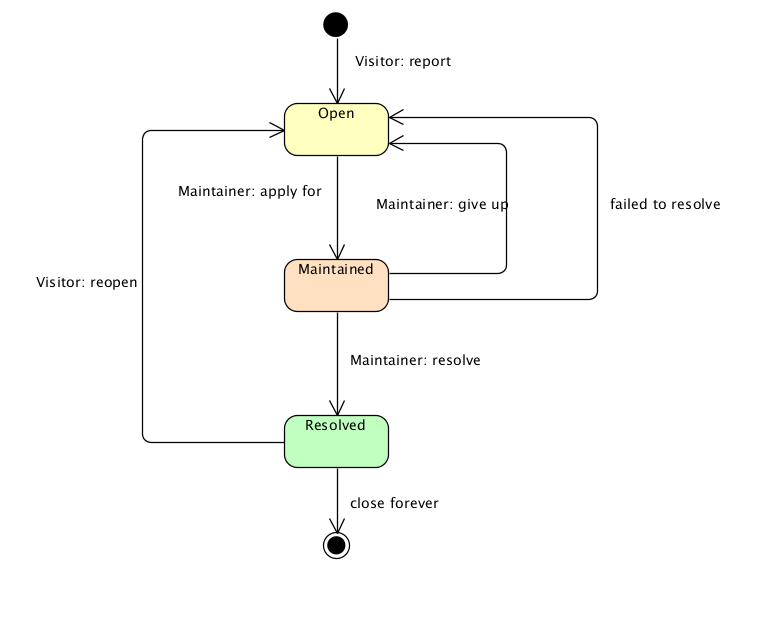
\includegraphics[width=75mm]{img/diagramy/StateMachine/bugtracker.png}
\end{figure}

\end{frame}


%%%%%%%%%%%%%%%%%%%%%%%%%%%%%%%%%%%%%%%%%%%%%%%%%%%%%%%%%%%%%%%%%%%%%%%%
